\section{Modifica di un progetto} \label{editor}
La pagina per la modifica di un \gloxy{progetto} permette all'utente di creare e modificare la \gloxy{mappa mentale} che sta alla base della presentazione e di definire vari \gloxy{percorsi di presentazione} ad essa associati che descrivono l'ordine in cui i contenuti dei nodi dovranno essere visualizzati durante la presentazione.\\
Al caricamento della pagina l'utente troverà il grafo che rappresenta la mappa mentale.\\
I nodi del grafo possono contenere vari elementi, sia testuali che grafici, che verranno utilizzati per la creazione dei \gloxy{frame} di presentazione.\\
Questi nodi sono collegati fra loro da relazioni gerarchiche (associazioni di tipo padre-figlio) e associazioni logiche, associazioni create dall'utente che mettono in evidenza il collegamento concettuale presente tra due nodi. \\
L'utente troverà nella pagina tutti gli strumenti necessari per poter creare la propria mappa mentale, definire associazioni logiche fra nodi e definire \gloxy{percorsi di presentazione} relativi alla mappa creata.\\
La pagina è formato da due viste, che sono \textit{Modifica mappa} e \textit{Modifica \gloxy{percorsi}}.
Queste due viste permettono di usufruire rispettivamente degli strumenti per la modifica della \gloxy{mappa mentale} e degli strumenti per modifica \gloxy{percorsi} dei \gloxy{percorsi}.\\
L'utente può passare da una vista all'altra tramite i pulsanti \textbf{\textit{Mappa}} e \textbf{\gloxy{Percorsi}} presenti al centro della barra di intestazione dell'applicazione.\\
La barra di intestazione contiene anche altri pulsanti che permettono di modificare la visualizzazione della \gloxy{mappa mentale} e di modificare le impostazioni del \gloxy{progetto}.
\begin{figure}[H]
\centering
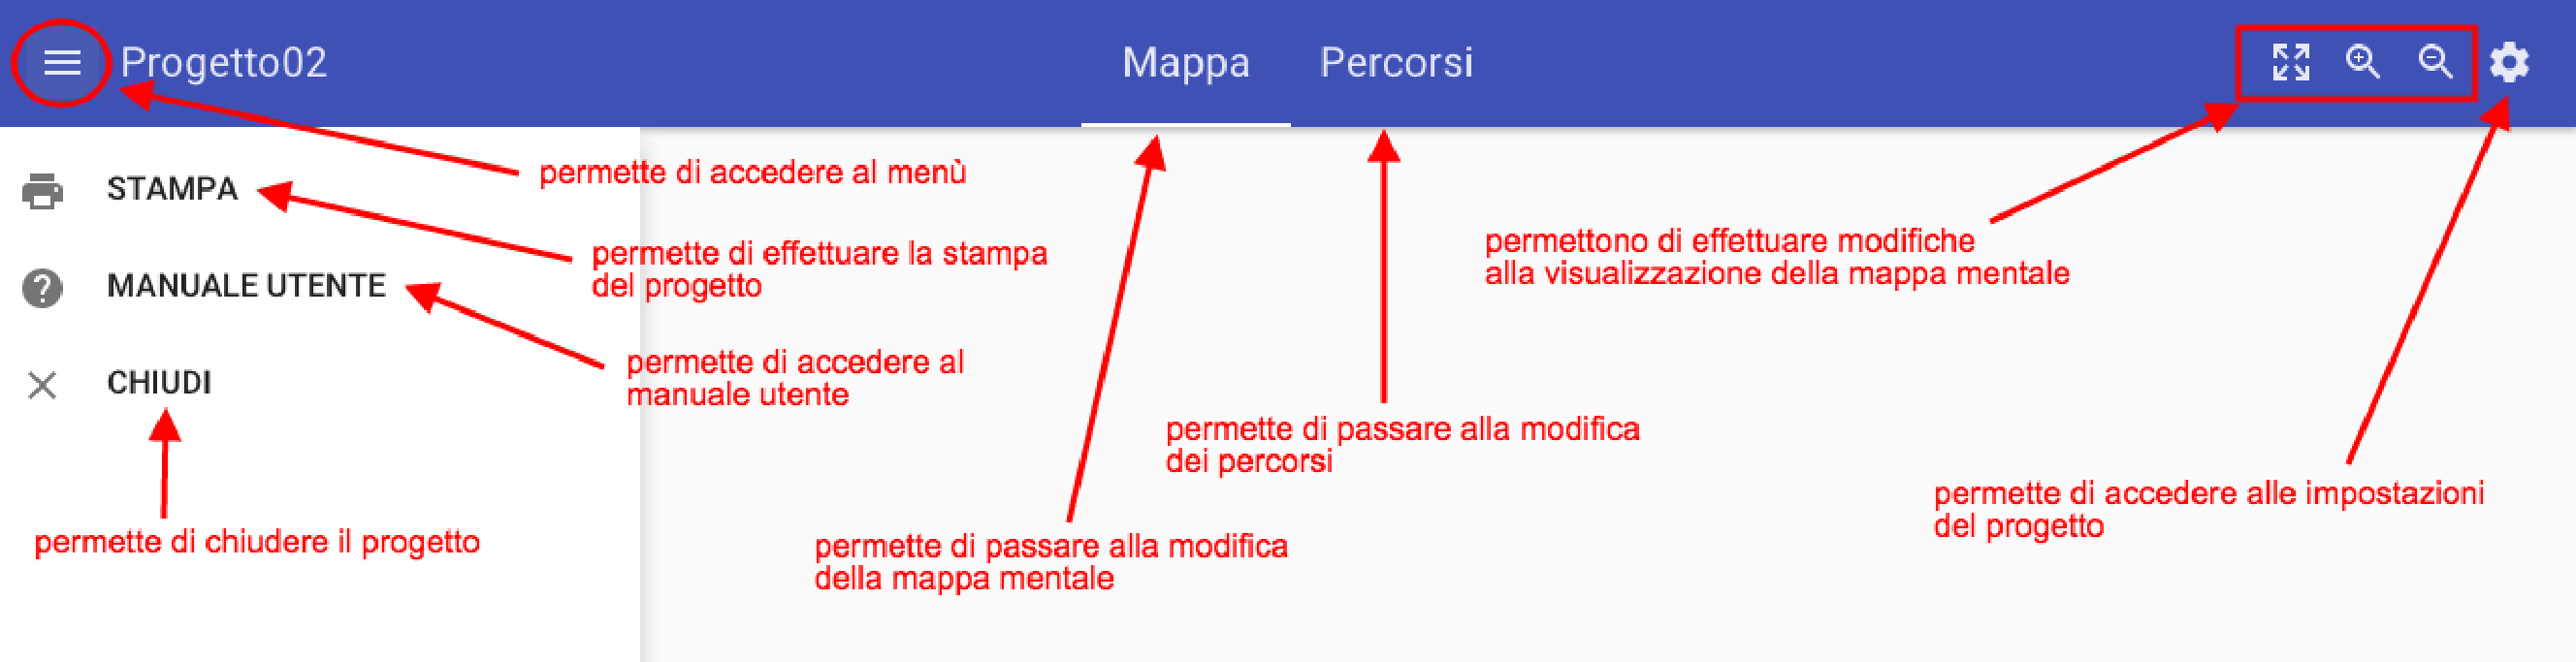
\includegraphics[scale=0.32]{immagini/strumentiHeader.pdf}
\caption{Pulsanti presenti nella barra di intestazione}
\end{figure}
Se il \gloxy{progetto} aperto è appena stato creato, l'utente troverà un nodo già esistente. Questo è il nodo \textit{radice} e rappresenta il nodo base della mappa mentale. L'utente potrà iniziare la creazione della mappa partendo da questo nodo.
\subsection{Modifica della mappa mentale}
\begin{figure}[H]
\centering
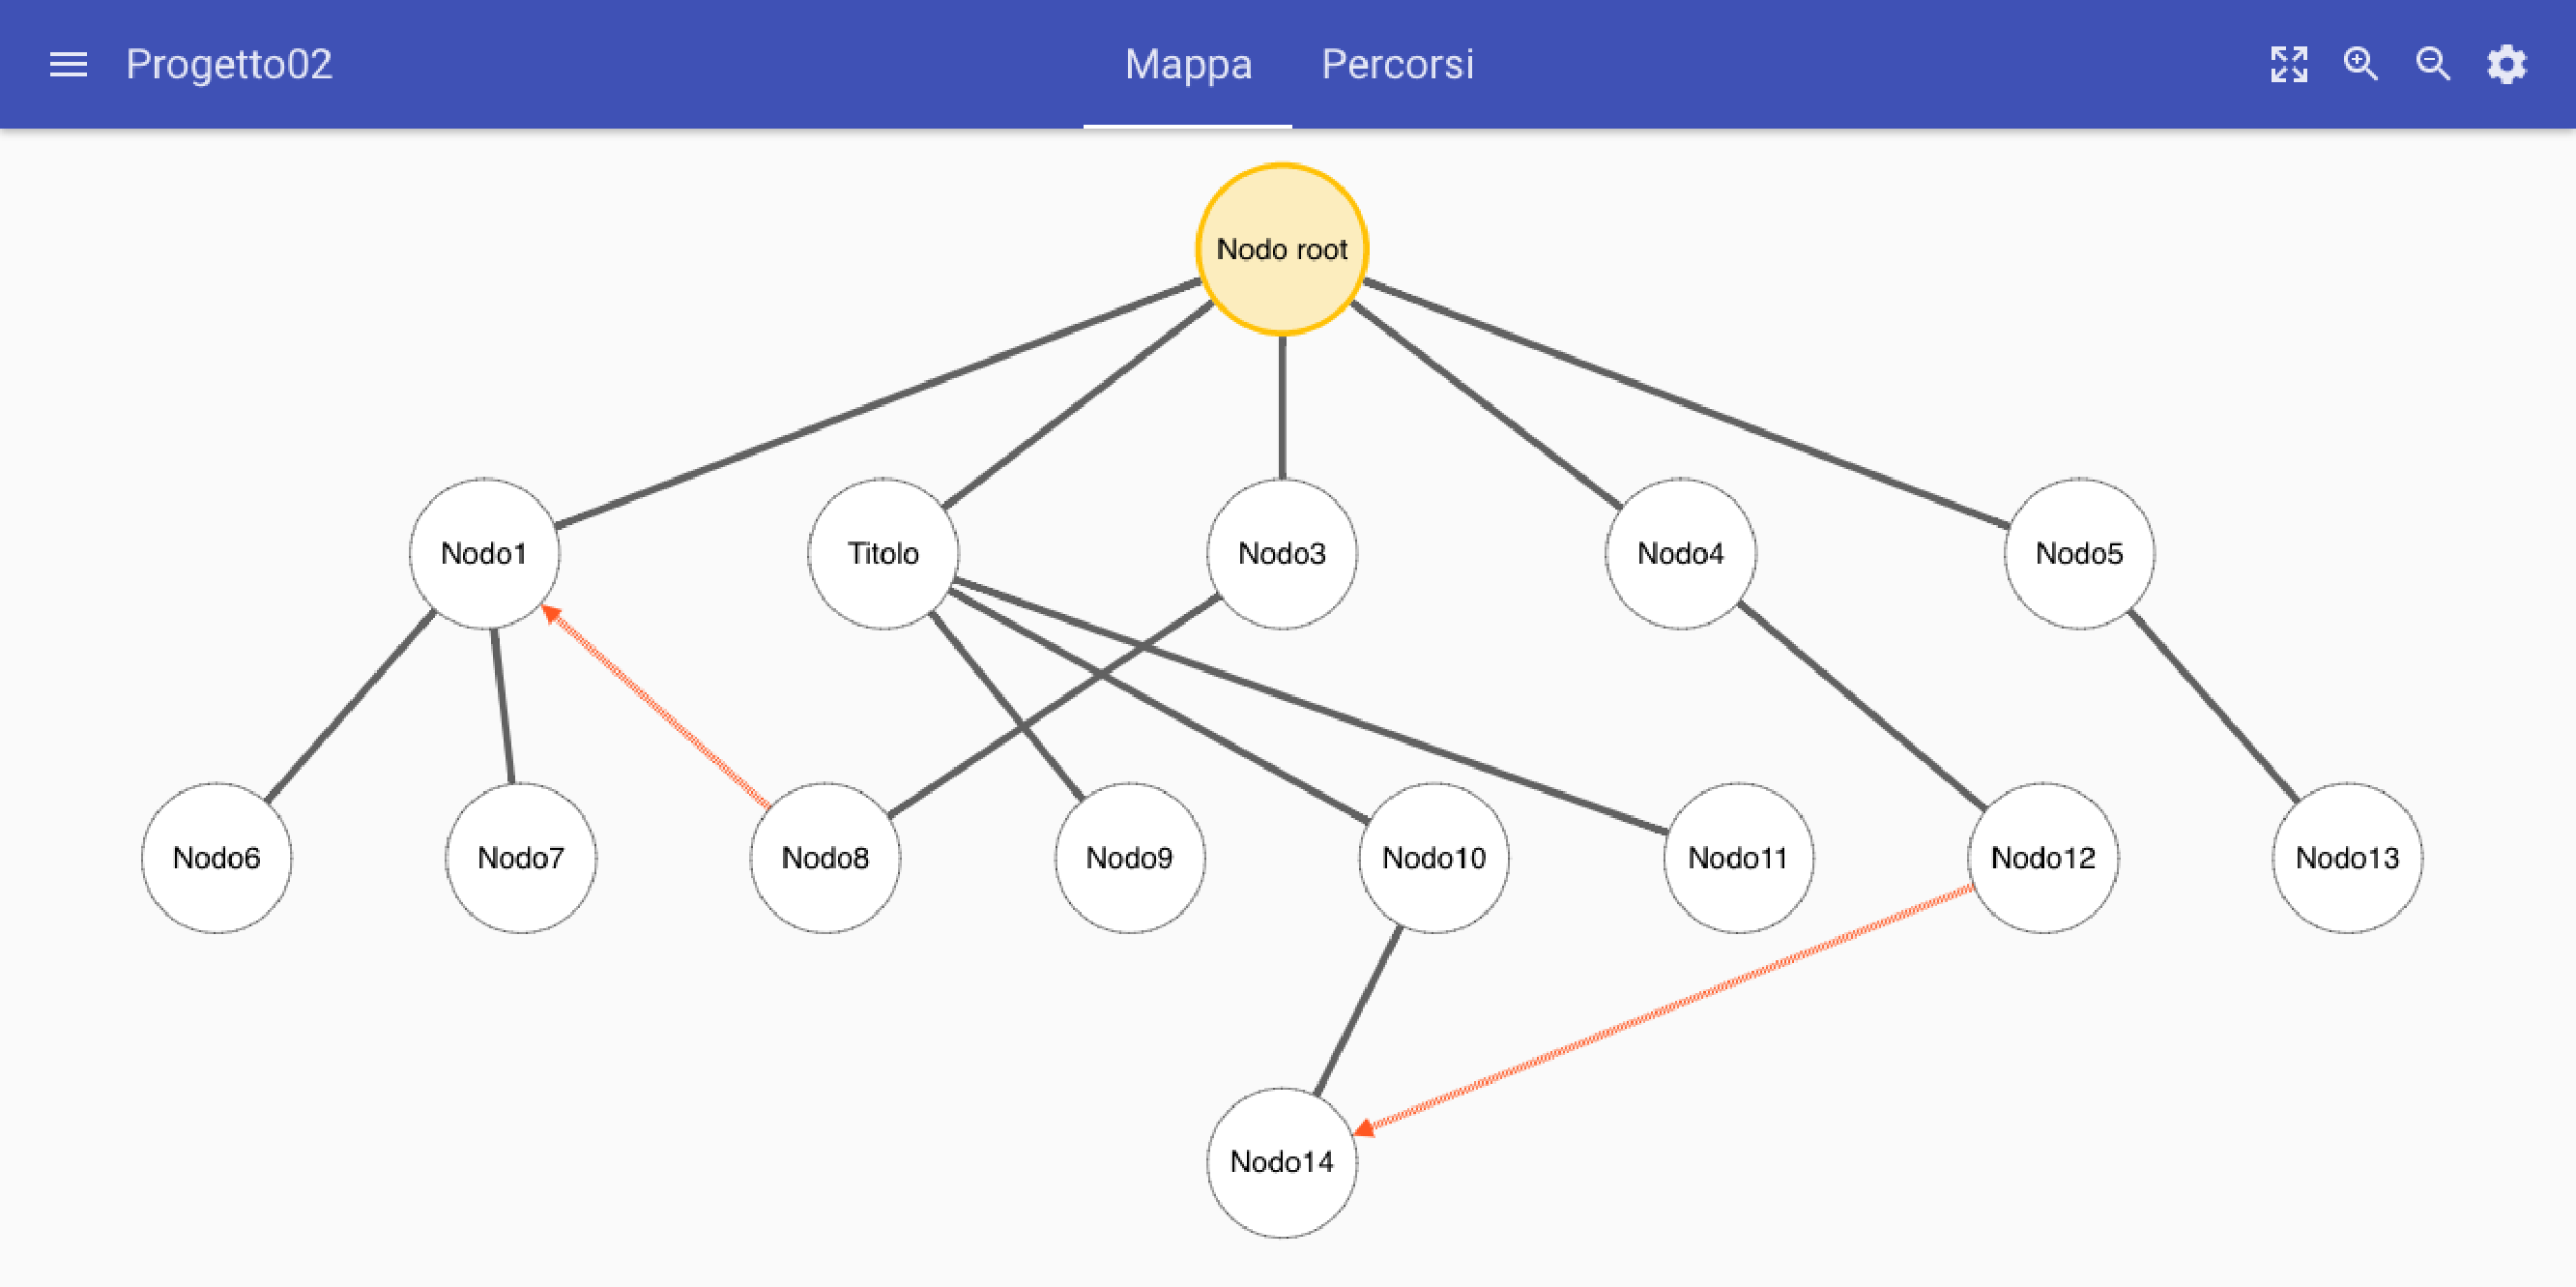
\includegraphics[scale=0.3]{immagini/modificaMappa.pdf}
\caption{Pagina per la modifica della mappa mentale}
\end{figure}
\FloatBarrier
Verranno descritti in seguito gli strumenti che l'utente potrà utilizzare per manipolare la \gloxy{mappa mentale} che desidera creare.

\subsubsection{Spostamento dei nodi}
Per poter spostare un nodo, l'utente deve effettuare il \textit{drag and drop} del nodo nella posizione desiderata. Questa modifica è temporanea dato che la disposizione dei nodi viene calcolata in modo automatico dall'applicazione.

\begin{figure}[H]
\centering
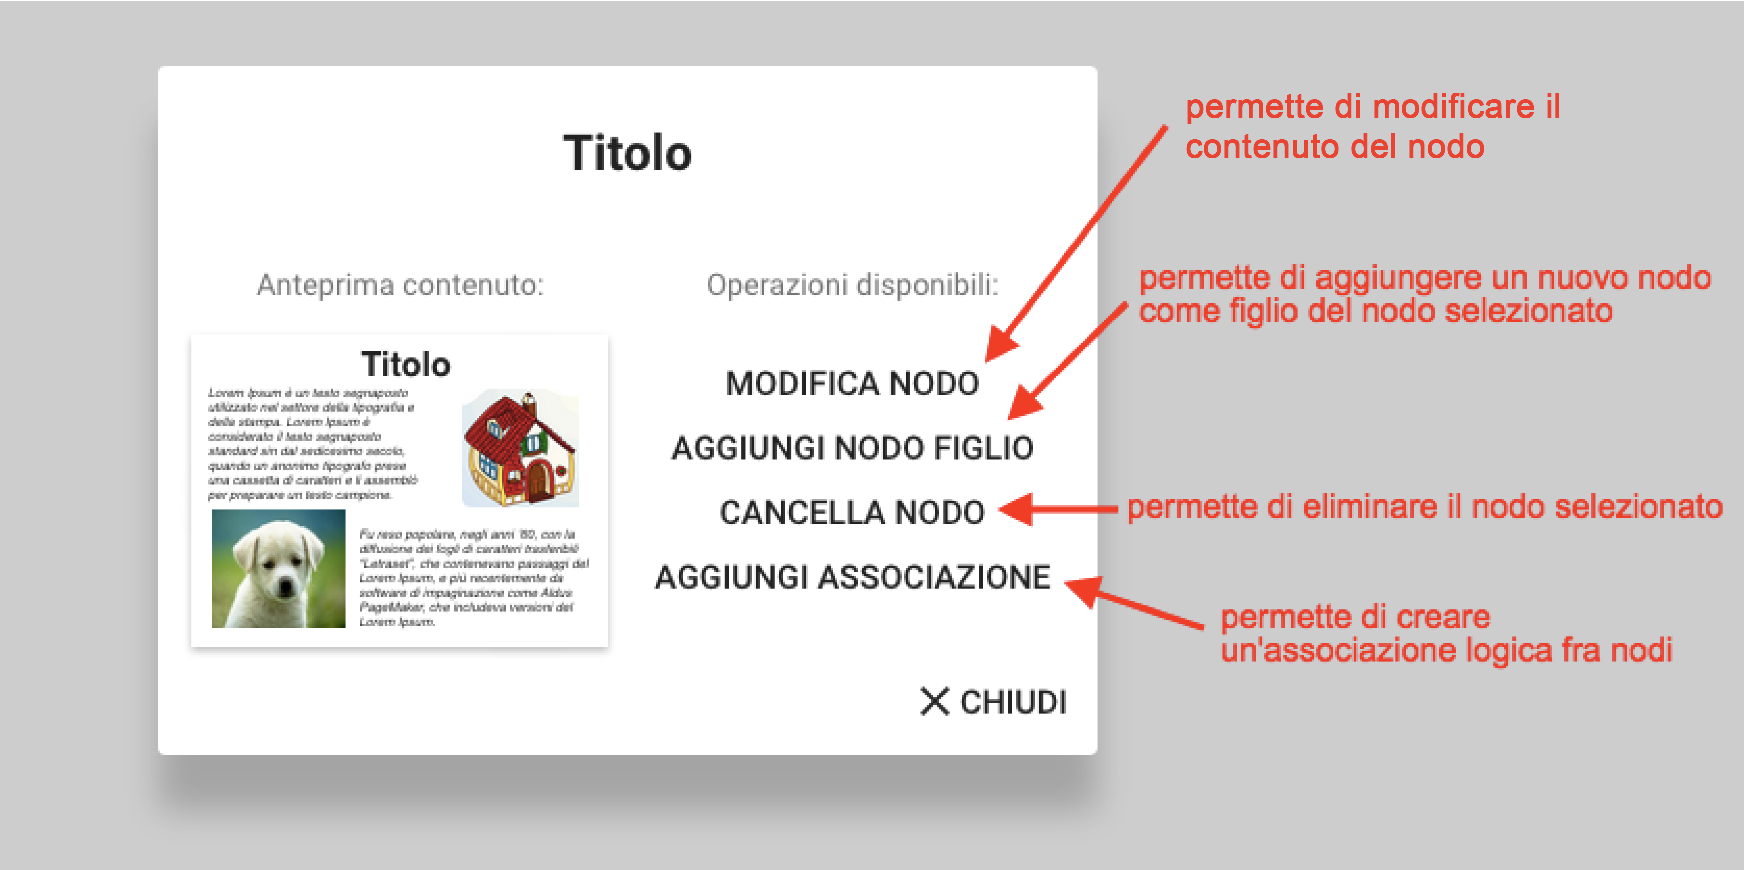
\includegraphics[scale=0.5]{immagini/menuNodoMappa.pdf}
\caption{Menù nodo nella fase di modifica mappa \label{menuNodoMappa}}
\end{figure}
\subsubsection{Creazione nuovo nodo}
Per creare un nuovo nodo, l'utente deve selezionare il nodo a cui desidera aggiungere il nuovo nodo figlio.\\
Verrà visualizzata una nuova finestra contenente un'anteprima dei contenuti del nodo e un elenco delle azioni disponibili. L'utente dovrà selezionare dal menù la voce \textbf{\textit{Aggiungi nodo figlio}}. Una volta premuto il pulsante, il sistema creerà in automatico un nuovo nodo vuoto come figlio del nodo selezionato.
\subsubsection{Eliminazione di un nodo}
Per poter eliminare un nuovo nodo, l'utente deve cliccare sul nodo che desidera eliminare.\\
Verrà visualizzata una nuova finestra contenente un'anteprima dei contenuti del nodo e un elenco delle azioni disponibili. L'utente dovrà selezionare dal menù la voce \textbf{\textit{Cancella nodo}}.\\
Se il nodo che si vuole cancellare ha dei figli o delle associazioni con altri nodi, verranno anchesse cancellate.\\
\subsubsection{Creazione di associazioni logiche}
Per poter creare un'\textit{associazione logica} tra due nodi, l'utente deve:
\begin{enumerate}
\item Selezionare il nodo origine dell'associazione;
\item Selezionare dal menù la voce \textbf{Aggiungi associazione};
\item Dalla finestra che comparirà, selezionare la voce \textbf{seleziona nodo}, per visualizzare la lista dei nodi associabili;
\item Selezionare dalla lista il nodo con cui creare l'associazione;
\item Premere il pulsante di conferma.
\end{enumerate}
L'associazione logica verrà rappresentata tramite una freccia tratteggiata di colore arancio.
\begin{figure}[H]
\centering
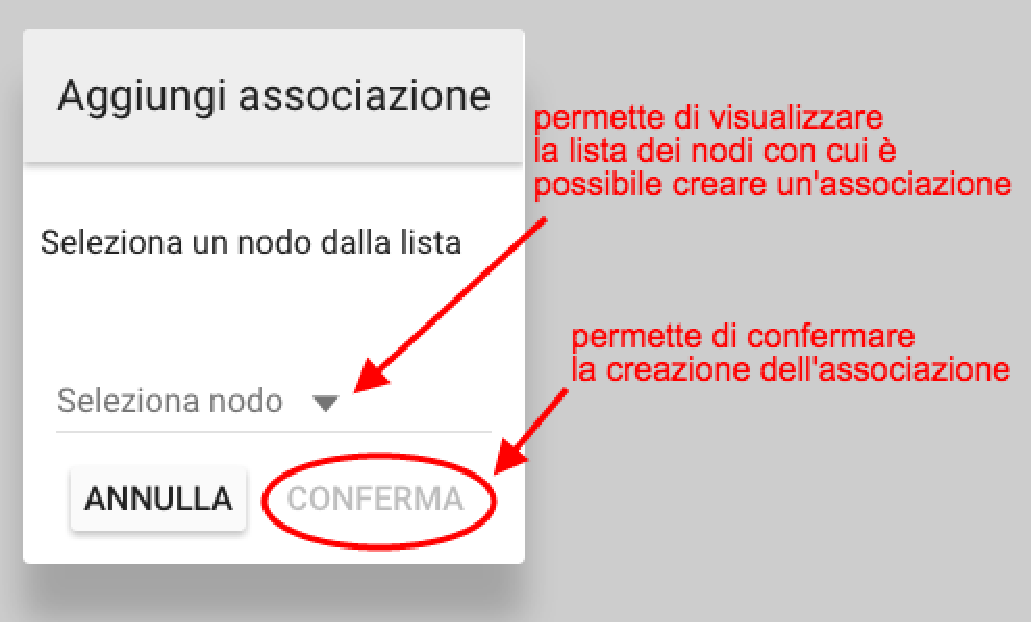
\includegraphics[scale=0.5]{immagini/associazioneMenu.pdf}
\caption{Menù delle associazioni logiche}
\end{figure}
\subsubsection{Eliminazione associazioni logiche}
Per poter eliminare un'\textit{associazione logica}, l'utente deve:
\begin{enumerate}
\item Selezionare l'associazione logica che desidera eliminare;
\item Selezionare la voce \textbf{\textit{cancella associazione}} dal menù che comparirà.
\end{enumerate}
\subsubsection{Inserimento contenuti}
Per poter inserire dei contenuti all'interno di un nodo, l'utente deve selezionare il nodo nel quale desidera inserire dei contenuti.\\
Verrà visualizzata una nuova finestra contenente un'anteprima dei contenuti del nodo e un elenco di azioni possibili. L'utente dovrà selezionare dal menù la voce \textbf{\textit{Modifica nodo}}.\\
Verrà visualizzata una nuova finestra nella quale sarà possibile gestire i contenuti del nodo, le varie funzionalità offerte verranno descritte nella sezione \nameref{editNodo}.
\subsection{Modifica del contenuto di un nodo}\label{editNodo}
In questa sezione verrà spiegato come utilizzare le funzionalità offerte dall'applicazione per gestire i contenuti di un nodo della mappa mentale.\\
La finestra mostra nella parte sinistra due pulsanti, che sono rispettivamente \textbf{\textit{Aggiungi testo}} e \textbf{\textit{Aggiungi immagine}} e, nella parte destra una rappresentazione del \gloxy{frame} con i suoi contenuti.\\
L'utente può selezionare i contenuti \textit{cliccandoci} sopra e vedrà apparire, sotto i pulsanti per l'inserimento di nuovi contenuti, una vista che permette di effettuare le modifiche sull'elemento selezionato.
\begin{figure}[H]
\centering
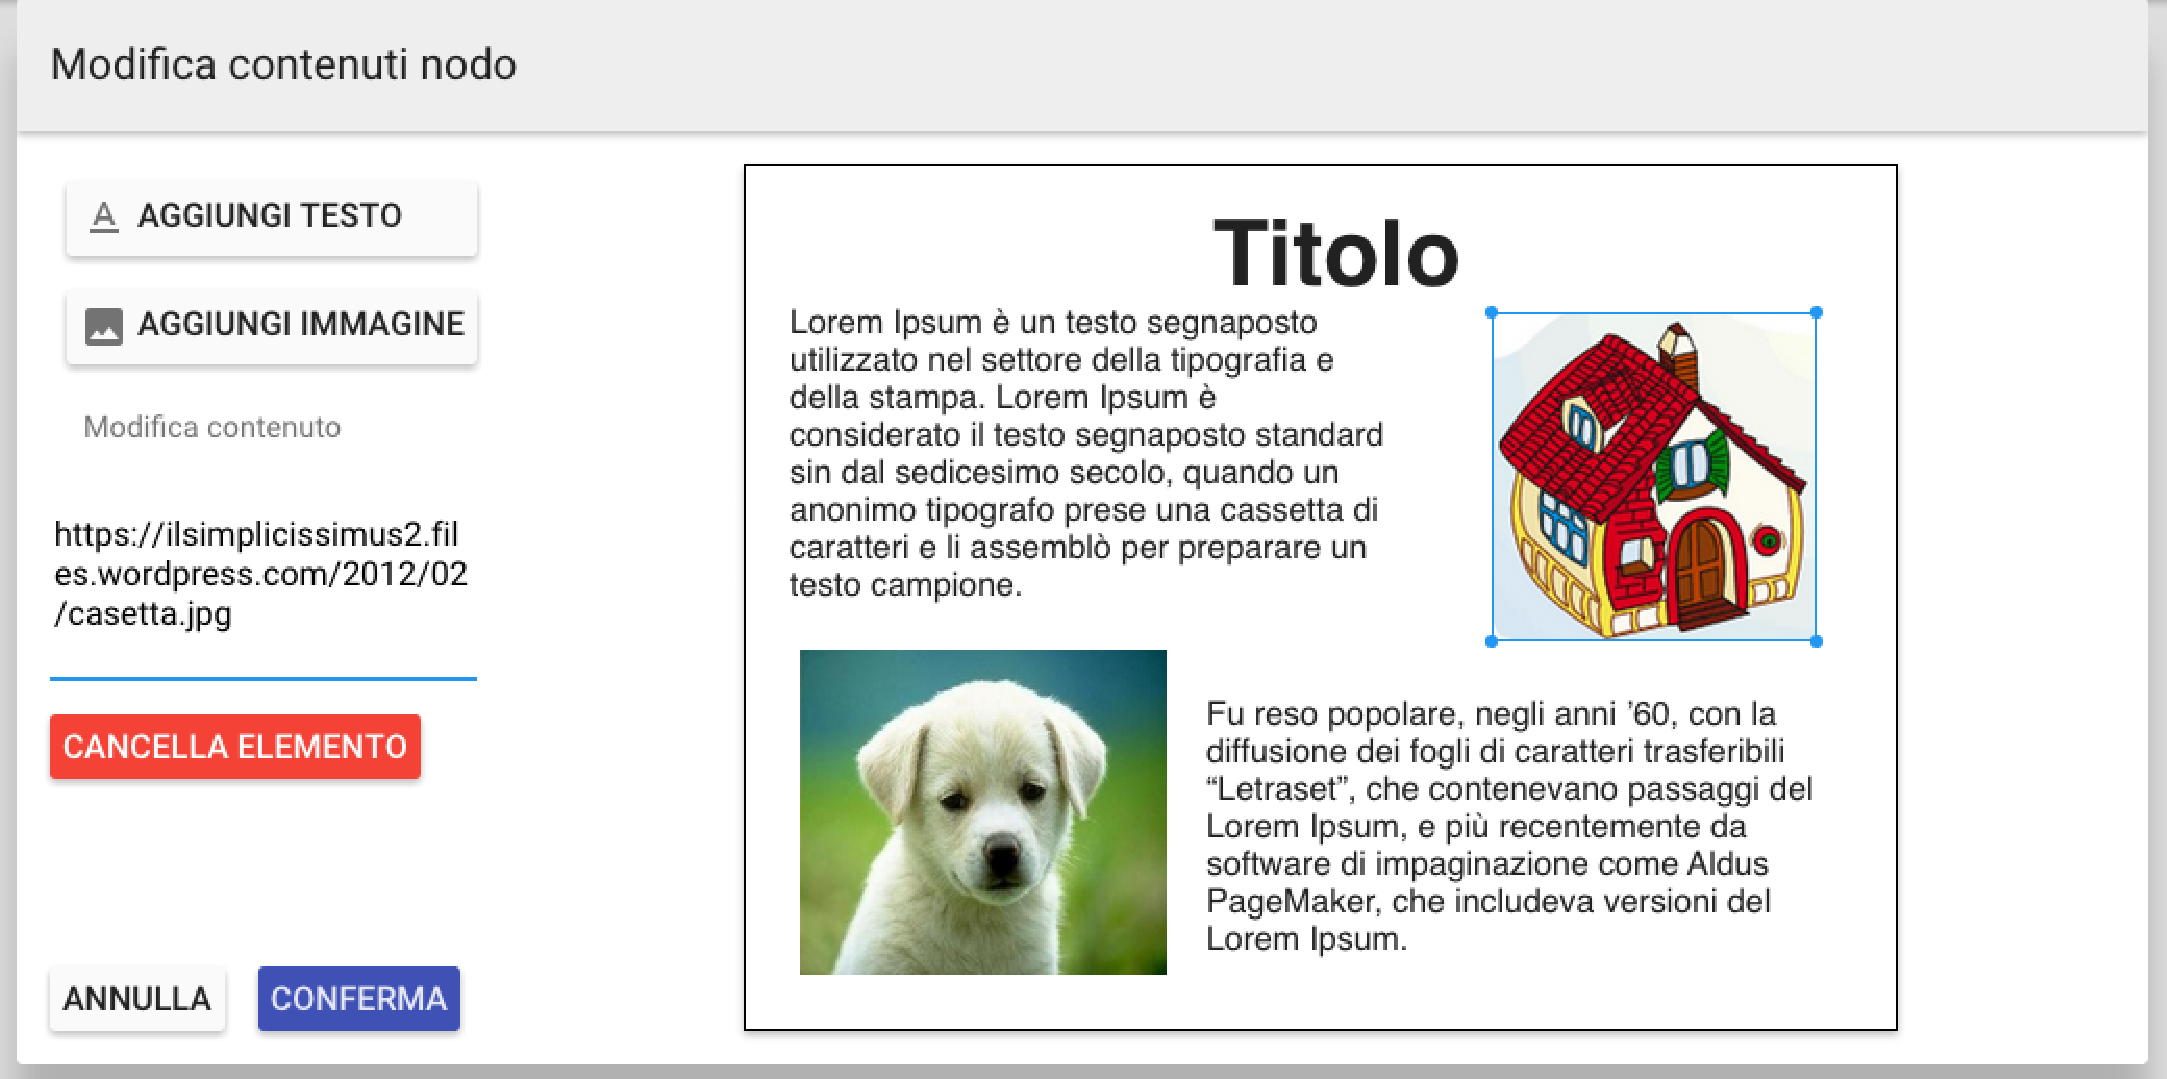
\includegraphics[scale=0.38]{immagini/modificaNodo.pdf}
\caption{Menù di modifica nodo \label{modificaNodo}}
\end{figure}
\subsubsection{Aggiungere del testo}
Per poter inserire del testo all'interno del nodo, l'utente deve premere il pulsante \textbf{\textit{Aggiungi testo}}, in questo modo verrà inserito all'interno del \gloxy{frame} un nuovo \textit{elemento testuale} contenente del testo di \textit{default}.\\
Per modificare il testo l'utente dovrà selezionare il nuovo elemento, in modo da rendere visibile lo strumento di modifica nella parte sinistra della finestra.
\subsubsection{Aggiungere un immagine}
Per poter inserire un'immagine all'interno del nodo, l'utente deve premere il pulsante \textbf{\textit{Aggiungi immagine}}, in questo modo verrà inserita all'interno del \gloxy{frame} un'immagine di default.
Per modificare l'immagine, l'utente dovrà selezionare il nuovo elemento e modificare l'URL in esso contenuto tramite lo strumento di modifica che diventerà visibile nella parte sinistra della finestra, inserendo l'URL della nuova immagine.\\
L'URL dell'immagine deve riferirsi ad un'immagine presente sul \textbf{\gloxy{web}}.
\subsubsection{Posizionamento contenuti}
Per poter posizionare un contenuto all'interno del \gloxy{frame}, l'utente dovrà trascinarlo, tramite \textit{drag and drop}, nella posizione desiderata.
\subsubsection{Ridimensionamento contenuto}
Per poter ridimensionare un contenuto, l'utente dovrà selezionare il contenuto che desidera ridimensionare e posizionandosi sui bordi del contenuto selezionato ridimensionarlo.
\subsection{Modifica dei percorsi di presentazione}
\begin{figure}[H]
\centering
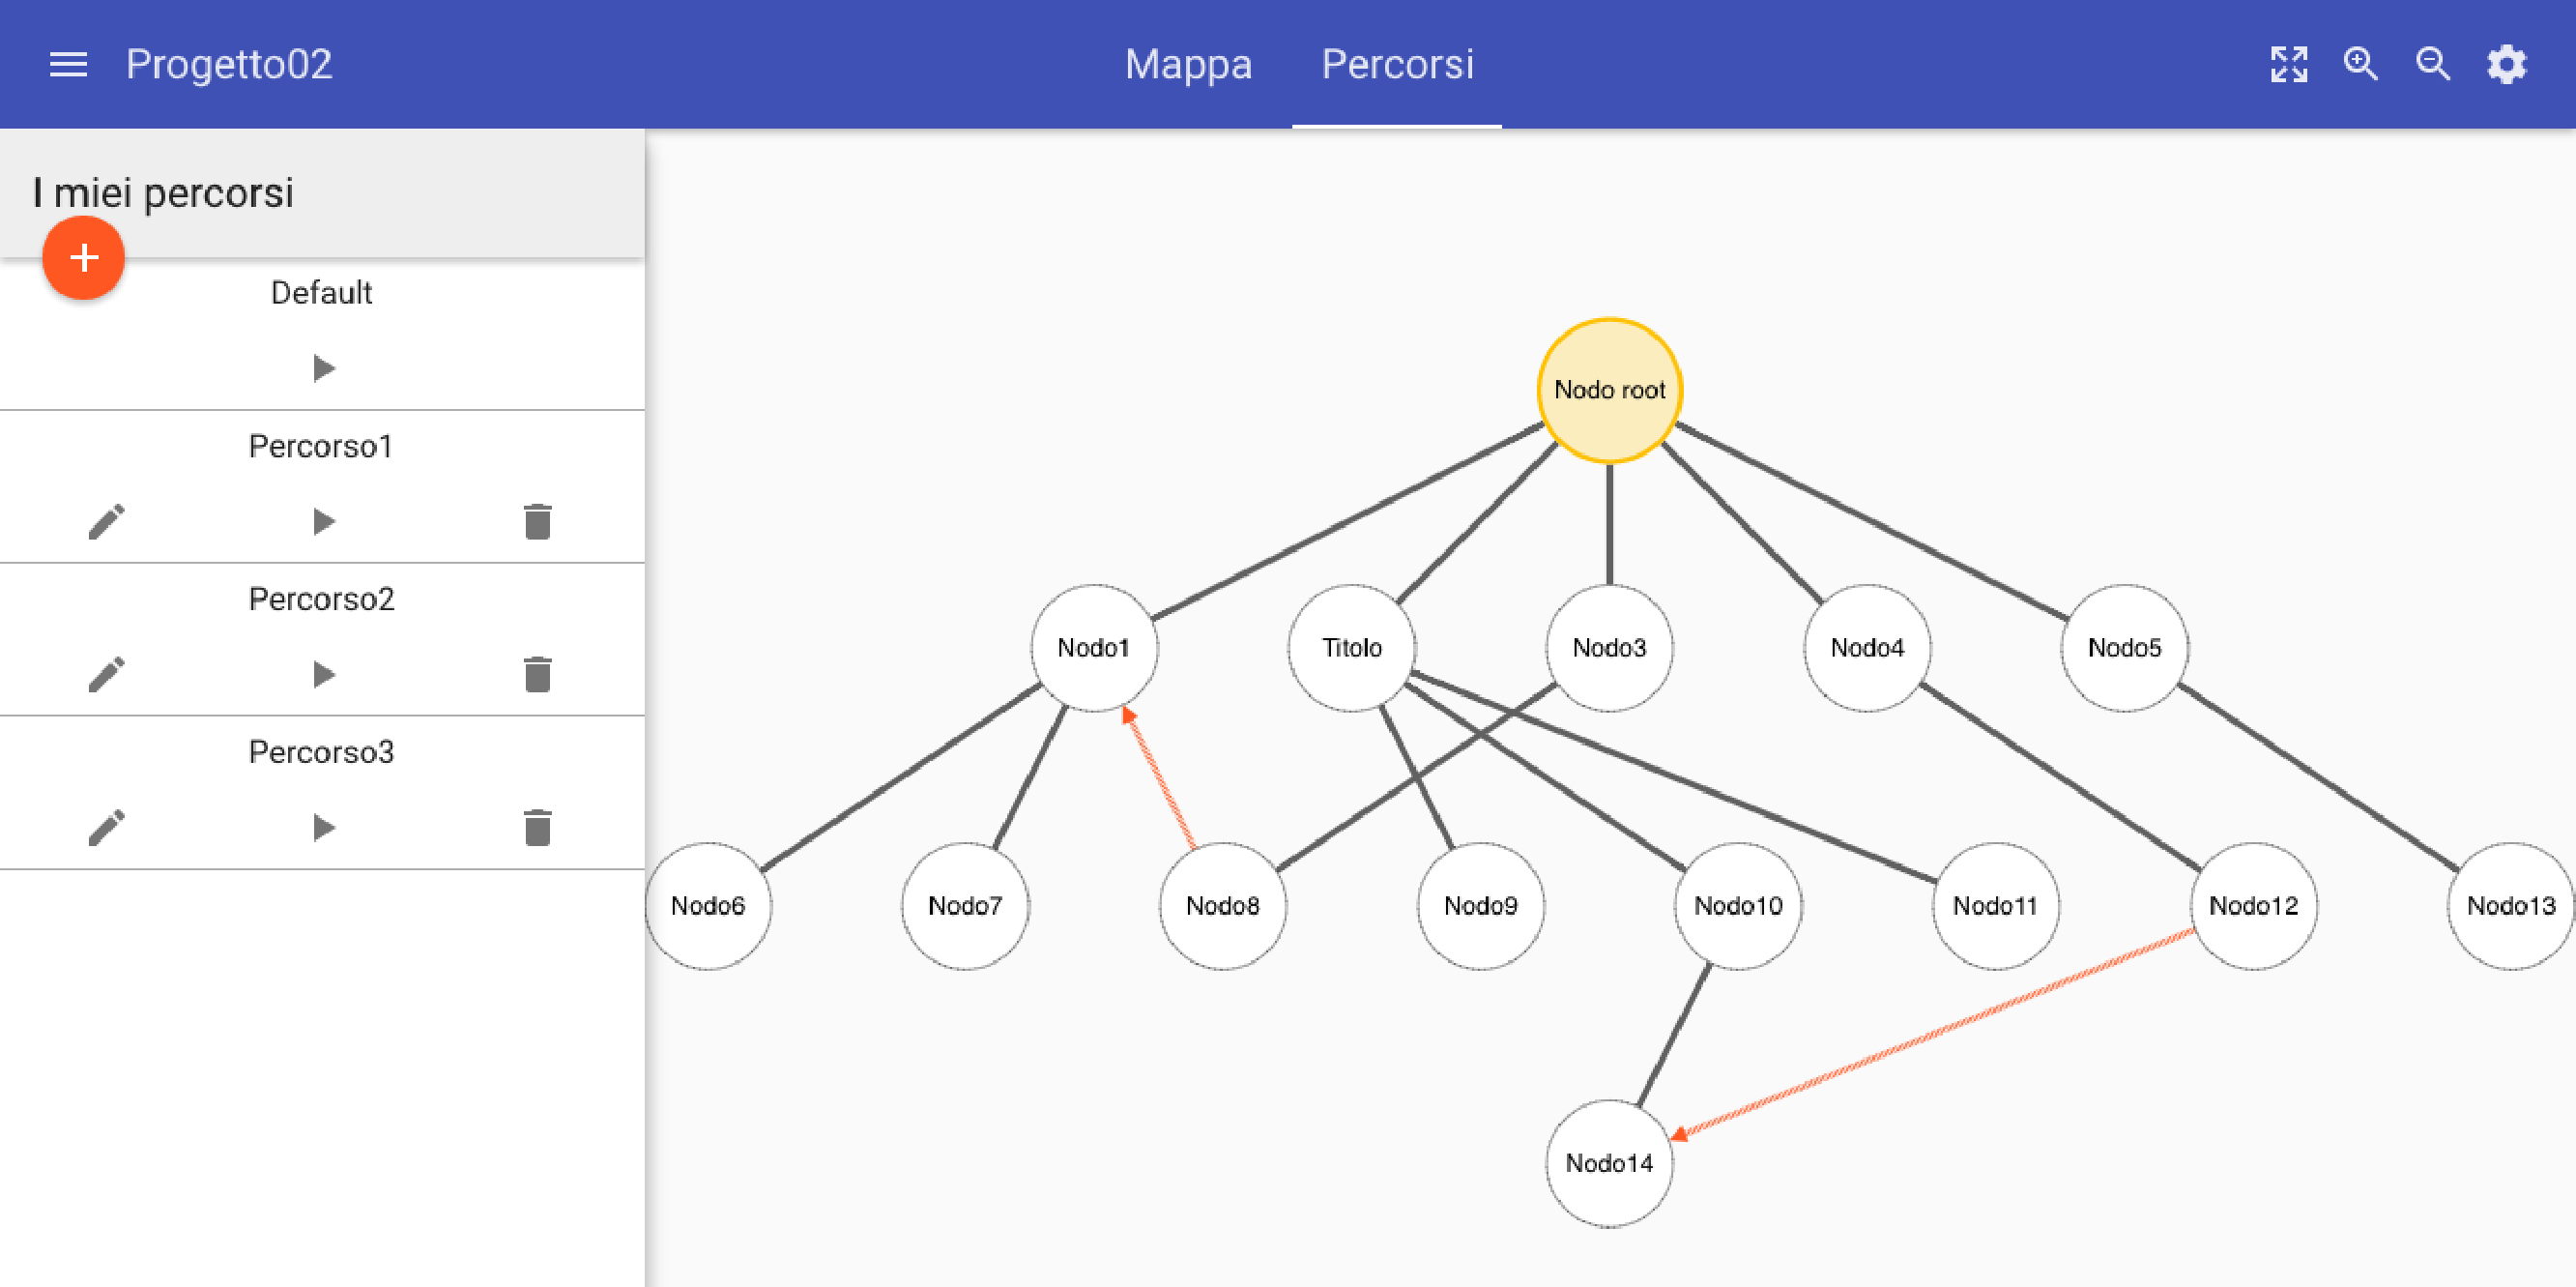
\includegraphics[scale=0.3]{immagini/modificaPercorsi.pdf}
\caption{Pagina per la modifica del percorsi}
\end{figure}
\FloatBarrier
Verranno descritte in seguito gli strumenti che l'utente potrà utilizzare per la creazione e la gestione dei \gloxy{percorsi} personalizzati di presentazione.
\subsubsection{Creazione nuovo percorso}
Per poter creare un nuovo \gloxy{percorso} di presentazione, l'utente deve trovarsi nella vista \textit{\gloxy{percorsi}} e deve premere il pulsante \textbf{più} 
\includegraphics[scale=0.5]{immagini/piuButton.pdf} presente nella parte sinistra della vista.
Verrà visualizzata una finestra, nella quale l'utente dovrà inserire il nome del nuovo \gloxy{percorso} e premere il pulsante \textbf{Aggiungi}.
\subsubsection{Modifica di un percorso}
Per poter modificare il nome di un \gloxy{percorso} ed il suo contenuto, l'utente deve premere il pulsante con l'icona rappresentante una matita presente nella lista \gloxy{percorsi} relativa al \gloxy{percorso} che desidera modificare.\\
Dalla finestra che compare l'utente potrà rinominare il \gloxy{percorso di presentazione} oppure rimuovere dei nodi dal \gloxy{percorso}.\\
Per il \gloxy{percorso} di default non è disponibile questa opzione.
%immagine della schermata
\begin{figure}[H]
\centering
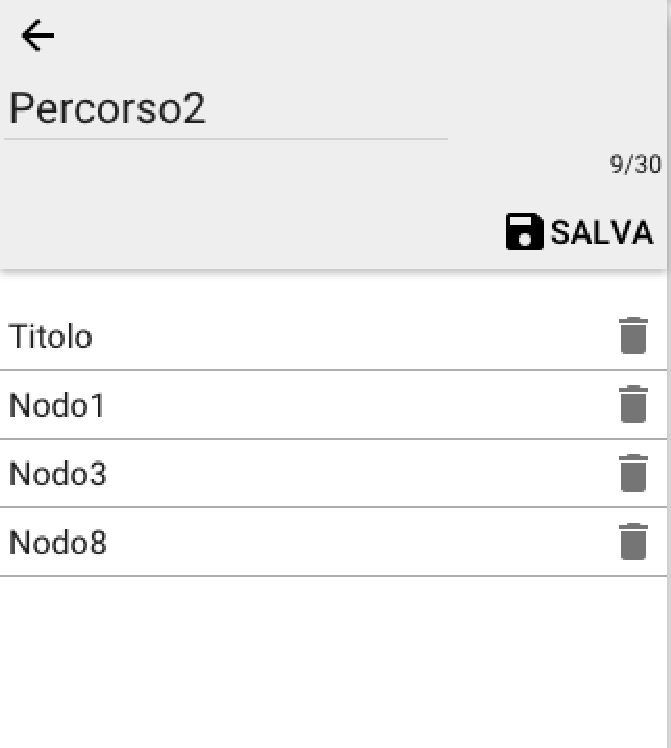
\includegraphics[scale=0.6]{immagini/modificaPercorso.pdf}
\caption{Modifica percorsi - lista dei nodi di un percorso}
\end{figure}
\FloatBarrier
\subsubsection{Eliminazione percorso}
Per poter eliminare un \gloxy{percorso}, l'utente deve premere il pulsante con l'icona rappresentante un cestino presente nella lista \gloxy{percorsi} e relativa al \gloxy{percorso} che desidera eliminare.\\
Per il \gloxy{percorso} di default non è disponibile questa opzione.
\begin{figure}[H]
\centering
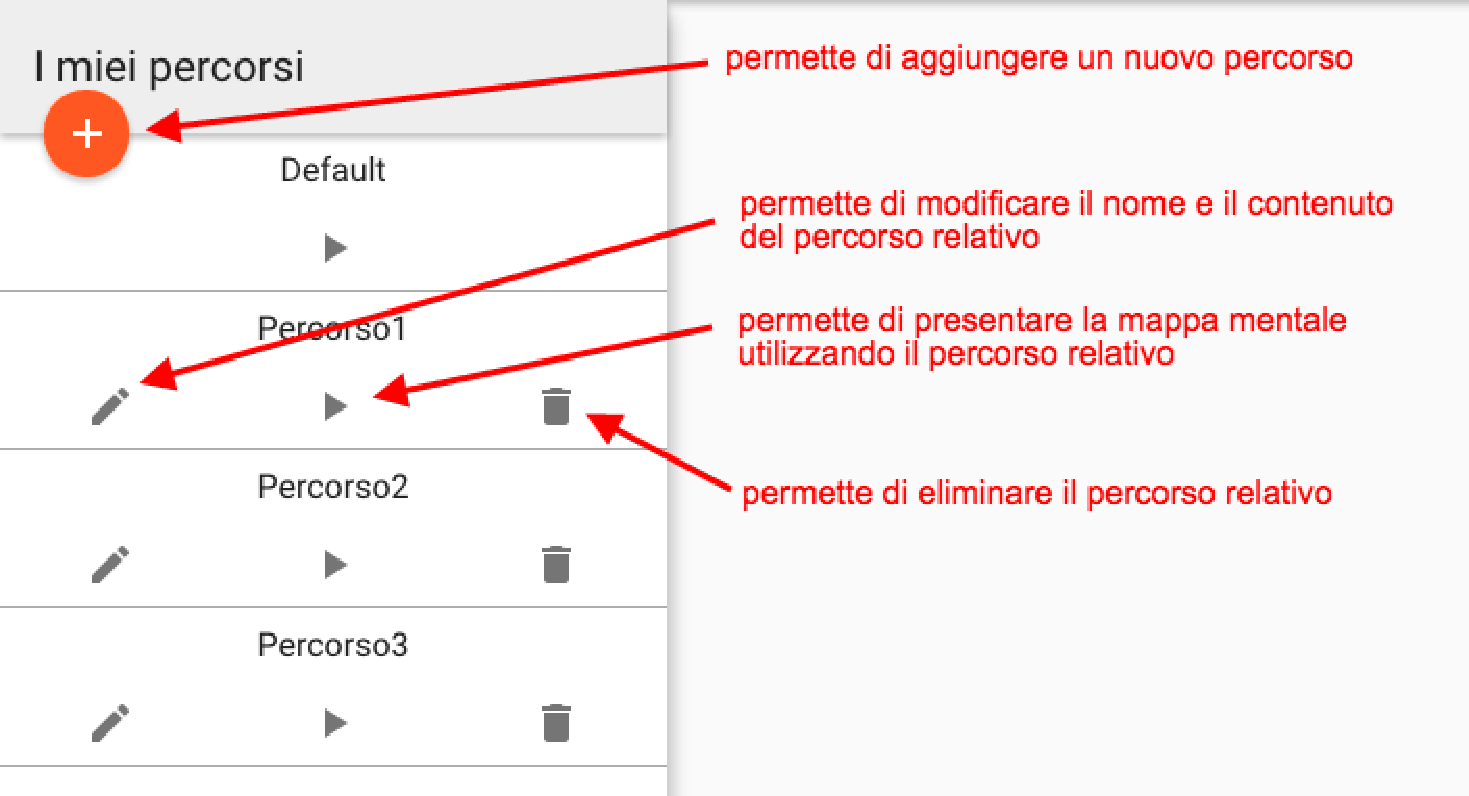
\includegraphics[scale=0.5]{immagini/menuPercorsi.pdf}
\caption{Modifica percorsi - lista dei percorsi}
\end{figure}
\subsubsection{Aggiunta di un nodo ad un percorso di presentazione}
Per poter aggiungere un nodo ad un \gloxy{percorso di presentazione} l'utente deve:
\begin{enumerate}
\item Trovarsi nella vista \textbf{\gloxy{Percorsi}};
\item Selezionare il nodo dalla mappa mentale;
\item Selezionare dalla finestra che comparirà, il \gloxy{percorso} al quale aggiungere il nodo selezionato.
\end{enumerate}
\begin{figure}[H]
\centering
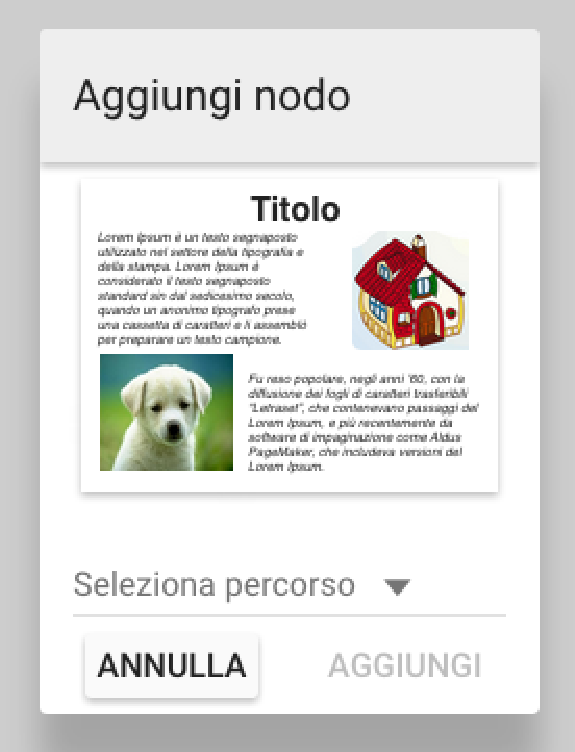
\includegraphics[scale=0.6]{immagini/aggiuntaNodoAPercorso2.pdf}
\caption{Aggiunta di un nodo ad un percorso di presentazione}
\end{figure}
\subsection{Modifica delle impostazioni del progetto}
Tramite questo strumento l'utente può effettuare delle modifiche al \gloxy{progetto} sul quale sta lavorando.\\ In particolare potrà modificare:
\begin{itemize}
\item Il nome del \gloxy{progetto};
\item Il colore di sfondo dei \gloxy{frame} del \gloxy{progetto};
\item Il colore del testo dei \gloxy{frame} del \gloxy{progetto};
\item Il font utilizzato nei \gloxy{frame} del \gloxy{progetto}.
\end{itemize}
La finestra \textbf{\textit{Impostazioni del }\gloxy{progetto}} può essere raggiunta premendo l'icona rappresentante un ingranaggio

\includegraphics[scale=0.5]{immagini/impostazioniButton.pdf}, presente all'interno della barra di intestazione dell'applicazione.
\begin{figure}[H]
\centering
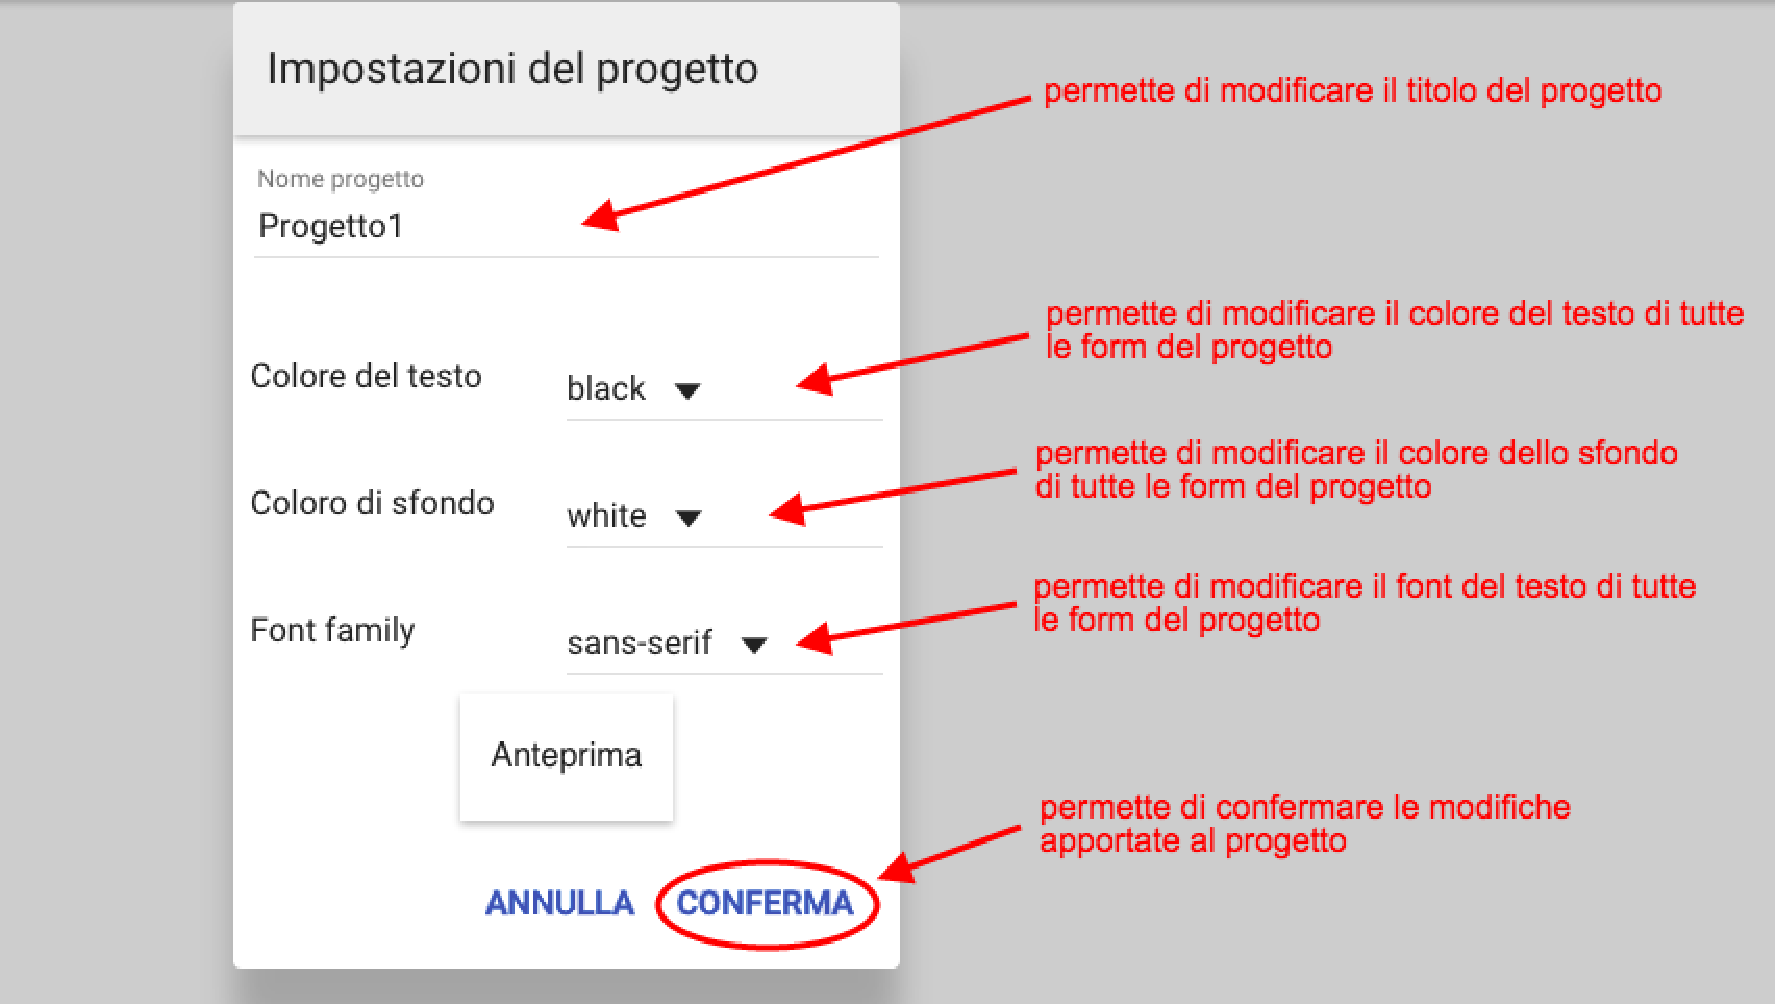
\includegraphics[scale=0.5]{immagini/impostazioneProgetto.pdf}
\caption{Impostazioni del progetto}
\end{figure}
